\documentclass{ximera}

\usepackage{float}

\newcommand{\R}{\mathbb R}

\newcommand{\href}[2]{#2\footnote{\url{#1}}}
\newcommand{\verticalvector}[1]{\begin{bmatrix}#1\end{bmatrix}}
\newcommand{\gt}{>}

\pgfplotsset{compat=1.8}
\graphicspath{
{./}
{introduction/}
{unit1/}
{unit1/theGeometryOfLinearEquations/}
{unit1/EliminationwithMatrices/}
{unit1/MultiplicationandInverseMatrices/}
}


\title{Elimination with matrices}

\begin{document}
\begin{abstract}
  Unit 1 MIT OCW Linear Algebra: Multiplication and Inverse Matrices
\end{abstract}
\maketitle

The MIT OCW Video Lecture can be found
here:\video{https://www.youtube.com/watch?v=FX4C-JpTFgY}\\

This lecture looks at matrix multiplication from five different points
of view. We then learn how to find the inverse of a matrix using elimination,
and why the Gauss-Jordan method works.

\begin{figure}[H]
\begin{image}
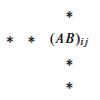
\includegraphics{1_3.jpg}
\end{image}
\end{figure}

\section*{Matrix Multiplication}

We discuss four different ways of thinking about the product $AB = C$ of two
matrices. If $A$ is an $m x n$ matrix and $B$ is an $n x p$ matrix, then $C$ is an $m x p$
matrix. We use $c_{ij}$ to denote the entry in row i and column j of matrix $C$.

\subsection*{Standard (row times column)}
The standard way of describing a matrix product is to say that $c_{ij}$ equals the dot
product of row i of matrix $A$ and column j of matrix $B$. In other words,

$c_{ij} = \sum\limits_{1}^{n} a_{ik}b_{kj}$

\subsection*{Columns}

The product of matrix $A$ and column j of matrix $B$ equals column j of matrix $C$.
This tells us that the columns of $C$ are combinations of columns of $A$.

\subsection*{Rows}

The product of row i of matrix $A$ and matrix $B$ equals row i of matrix $C$. So the rows
of $C$ are combinations of rows of $B$.

\subsection*{Column times row}

A column of $A$ is an $m x 1$ vector and a row of $B$ is a $1 x p$ vector. Their product
is a matrix:

\[
\begin{vmatrix} 2\\3\\4 \end{vmatrix} \cdot \begin{bmatrix} 1&6 \end{bmatrix} =
\begin{bmatrix}
2&12\\3&18\\4&24  
\end{bmatrix}
\]

The columns of this matrix are multiples of the column of $A$ and the rows are multiples
of the row of $B$. If we think of the entries in these rows as the coordinates $(2,12)$ or
$(3,18)$ or $(4,24)$, all these points lie on the same line; similarly for the two column
vectors. Later well see that this is equivalent to saying that the row space of this
matrix is a single line, as is the column space.

The product of $A$ and $B$ is the sum of these column times row matrices:

\[
AB = \sum\limits_{1}^{n} \begin{vmatrix} a_{1k}\\ \vdots \\a_{mk} \end{vmatrix}
\cdot \begin{bmatrix} b_{k1}&\cdots&b_{kn} \end{bmatrix}.
\]

\subsection*{Blocks}

If we subdivide $A$ and $B$ into blocks that match properly, we can write the 
product $AB = C$ in terms of products of the blocks:

\[
\begin{bmatrix} A_1&A_2\\A_3&A_4 \end{bmatrix} 
\begin{bmatrix} B_1&B_2\\B_3&B_4 \end{bmatrix} = \begin{bmatrix} C_1&C_2\\C_3&C_4 \end{bmatrix}
\]
here $C_1=A_1B_1 + A_2B_2$

\section*{Inverses}

\subsection*{Square matrices}

If $A$ is a square matrix, the most important question you can ask about it
is whether it has an inverse $A^{-1}$. If it does, then $A^{-1}A = I = AA^{-1}$
and we say that $A$ is invertible or nonsingular.

If $A$ is singular � i.e. $A$ does not have an inverse - its determinant is zero
and we can find some non-zero vector $x$ for which $Ax = 0$. For example:
\[
\begin{bmatrix} 1&3\\2&6 \end{bmatrix} \begin{vmatrix} \phantom{-} 3\\-1 \end{vmatrix} =
\begin{vmatrix} 0\\0 \end{vmatrix}.
\]
In this example, three times the first column minus one times the second column
equals the zero vector; the two column vectors lie on the same line.

Finding the inverse of a matrix is closely related to solving systems of linear equations:

\[
\begin{bmatrix} 1&3\\2&7 \end{bmatrix} \begin{bmatrix} a&c\\b&d \end{bmatrix} =
\begin{bmatrix} 1&0\\0&1 \end{bmatrix}
\]
\[A A^{-1} = I\]
can be read as saying $A$ times column $j$ of $A^{-1}$ equals column $j$ of the identity
matrix. This is just a special form of the equation $Ax = b$.


\section*{Gauss-Jordan Elimination}
We can use the method of elimination to solve two or more linear equations at the
same time. Just augment the matrix with the whole identity matrix $I$:

\[
\left[ \begin{array}{cc|cc} 1&3&1&0\\2&7&0&1 \end{array} \right] \rightarrow 
\left[ \begin{array}{cc|cc} 1&3&1&0\\0&1&-2&1 \end{array} \right] \rightarrow 
\left[ \begin{array}{cc|cc} 1&0&7&-3\\0&1&-2&1 \end{array} \right]
\]
(Once we have used Gauss elimination method to convert the original matrix to upper 
triangular form, we go on to use Jordans idea of eliminating entries in the upper 
right portion of the matrix.)

\[
A^{-1} = \begin{bmatrix} 7&-3\\-2&1 \end{bmatrix}.
\]

As in the last lecture, we can write the results of the elimination method as the
product of a number of elimination matrices $E_{ij}$ with the matrix $A$.
Letting $E$ be the product of all the $E_{ij}$, we write the result of this
Gauss-Jordan elimination using block matrices: $E[ A | I ] = [ I | E ]$.
But if $EA = I$, then $E = A^{-1}$.

\section*{Recitation}

\begin{question}
Find the conditions on $A$ and $B$ that make that matrix invertible, and find $A^{-1}$
when it exists:

\[
\begin{bmatrix} a&b&b\\a&a&b\\a&a&a \end{bmatrix}
\] 
\begin{solution}
\begin{hint}
The matrix is not invertible if a =\answer{0}
\end{hint}
\begin{hint}
$a=0$ as this would create an entire row of zeros which is always non-invertible.
\end{hint}

\begin{hint}
The matrix is not invertible if b=\answer{a}
\end{hint}
\begin{hint}
$b=a$ as this would create matrix where all the entries are identical or or all the rows
are the same, which as we said above is always non-invertible.
\end{hint}

\begin{hint}
You start by writing an augmented matrix that has $A$ and $I$ next to it. 
You perform elimination steps on this augmented matrix until you've reached the 
identity matrix on the left side. When you do that, what you have on the right 
side will be your A inverse.

\[
[A|I] \rightarrow [I|A^{-1}]
\]
\end{hint}

\begin{hint}
The Augmented Matrix is 
\begin{matrixAnswer}[name=M]
      The matrix is  [['a','b','b', '1', '0', '0'],['a','a','b', '0', '1', '0'],
      ['a','a','a', '0', '0', '1']]
\end{matrixAnswer}
\end{hint}

\begin{hint}
\[
A^{-1} = \frac {1}{a-b} \begin{bmatrix} \phantom{-}1&\phantom{-}0&-\frac{b}{a}\\-1&
\phantom{-}1&\phantom{-}0\\\phantom{-}0&-1&\phantom{-}1 \end{bmatrix}
\]
\end{hint}

\begin{matrixAnswer}[name=M]
      The matrix is  \frac {1}{a-b}[['1','0','-\frac{b}{a}'],['-1','1','0'],['0','-1','1']]
\end{matrixAnswer}

\end{solution}
\end{question}

The MIT Recitation video for this question is here:
here:\video{https://www.youtube.com/watch?v=xCIXkm3-ocQ}

\section*{Homework}

\begin{question}

Add Matrices $AB$ to $AC$ and compare with $A(B + C)$

\[
A= \begin{bmatrix}1&2\\3&4\end{bmatrix} B= \begin{bmatrix}1&0\\0&0\end{bmatrix}
C= \begin{bmatrix}0&0\\5&6\end{bmatrix}
\]

\begin{solution}

\begin{matrixAnswer}[name=M]
      AB = [['1','0'],['3','0']]      
\end{matrixAnswer}
\begin{matrixAnswer}[name=M]
      AC = [['10','12'],['20','24']]      
\end{matrixAnswer}
\begin{matrixAnswer}[name=M]
      AB + AC = [['11','12'],['23','24']]
\end{matrixAnswer}

Now Do $A(B+C)$
\begin{matrixAnswer}[name=M]
      B + C = [['1','0'],['5','6']]
\end{matrixAnswer}
\begin{matrixAnswer}[name=M]
      A(B + C) = [['11','12'],['23','24']]
\end{matrixAnswer}

Therefore, $AB + AC = A(B + C)$

\end{solution}
\end{question}

\begin{question}
(2.5 24. Introduction to Linear Algebra: Strang) Use Gauss-
Jordan elimination on $[U I]$ to find the upper triangular $U^{-1}$

\[
U = \begin{bmatrix}1&a&b\\0&1&c\\0&0&1\end{bmatrix}
\]

\begin{solution}

\begin{hint}
\[
%%The Augmented Matrix is $\begin{bmatrix}1&a&b&1&0&0\\0&1&c&0&1&0\\0&0&1$0&0&1\end{bmatrix}$
\]
\end{hint}
\[
The result is:
\begin{matrixAnswer}[name=M]
      [['1','0', '0', '1', '-a', 'ac-b'],['0','1', '0', '0', '1', '-c'],
       ['0', '0', '1', '0', '0', '1']]
\end{matrixAnswer}

\]
\end{solution}
\end{question}

\end{document}
